\subsection{Vertical velocity closure}
The hydrostatic momentum equations are written in terms of horizontal velocities, combined with mass conservation over the water column. Often it is necessary to recover the compatible conservative 3D velocity field, either for diagnostic purposes or to feed into the transport equations. 

SELFE infers vertical velocities by integrating the 3D mass conservation equation (\ref{3Dcon})
from the bed to the free surface. The process is illustrated in Figure \ref{fig:vel_close}. Starting at the bed, a suitable boundary condition (e.g. zero flow) is assumed. This is combined with horizontal flows across the three vertical faces of the prism as well as the component of flow flows directed across the (very slightly tilted) top face of the
prism. Given that water is incompressible, what comes out must be the vertical component of flow up out of the top face. The
calculation then proceeds to the prism above.

\begin{figure}
	\centering
		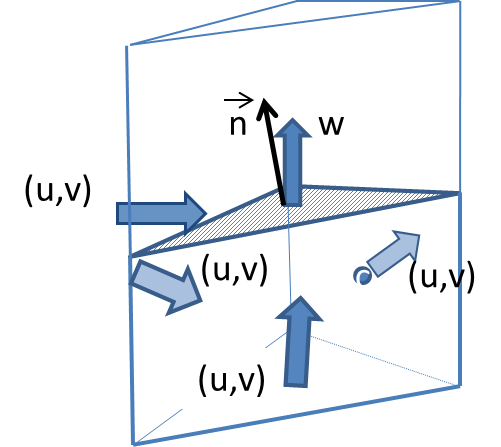
\includegraphics[scale=1.0]{image/vel_closure}
	\caption{First closure calculation on bottom prism. The horizontal velocities at the three vertical faces and the horzizontal component of velocity normal to the top face are shown and designated $(u,v)$. The vertical velocity $w$ is obtained from the 
	net flux. Movement of the S grid (typically a small fraction of a millimeter per time step) is not considered.}
	\label{fig:vel_close}
\end{figure}